
%%%%%%%%%%%%%%%%%%%%%%%%%%%%%%%%%%%%%%%%%%%%%%%%%%%%%%%%%%%%%%%%%%%%%%%%%%%%%%%%%%%%%%%
%%%%%%%%%%%%%%%%%%%%%%%%%%%%%%%%%%%%%%%%%%%%%%%%%%%%%%%%%%%%%%%%%%%%%%%%%%%%%%%%%%%%%%%
% 
% This top part of the document is called the 'preamble'.  Modify it with caution!
%
% The real document starts below where it says 'The main document starts here'.

\documentclass[12pt]{article}
\usepackage{hyperref}

\usepackage{amssymb,amsmath,amsthm}
\usepackage[top=1in, bottom=1in, left=1.25in, right=1.25in]{geometry}
\usepackage{fancyhdr}
\usepackage{enumerate}
\usepackage{listings}
\usepackage{graphicx}
\usepackage{float}
\usepackage{multicol}
% Comment the following line to use TeX's default font of Computer Modern.
\usepackage{times,txfonts}
\usepackage{mwe}
\usepackage{caption}
\usepackage{subcaption}

\usepackage{tikz}
\def\checkmark{\tikz\fill[scale=0.4](0,.35) -- (.25,0) -- (1,.7) -- (.25,.15) -- cycle;} 



\makeatletter
\renewcommand*\env@matrix[1][*\c@MaxMatrixCols c]{%
  \hskip -\arraycolsep
  \let\@ifnextchar\new@ifnextchar
  \array{#1}}
\makeatother

\newtheoremstyle{homework}% name of the style to be used
  {18pt}% measure of space to leave above the theorem. E.g.: 3pt
  {12pt}% measure of space to leave below the theorem. E.g.: 3pt
  {}% name of font to use in the body of the theorem
  {}% measure of space to indent
  {\bfseries}% name of head font
  {:}% punctuation between head and body
  {2ex}% space after theorem head; " " = normal interword space
  {}% Manually specify head
\theoremstyle{homework} 

% Set up an Exercise environment and a Solution label.
\newtheorem*{exercisecore}{\@currentlabel}
\newenvironment{exercise}[1]
{\def\@currentlabel{#1}\exercisecore}
{\endexercisecore}

\newcommand{\localhead}[1]{\par\smallskip\noindent\textbf{#1}\nobreak\\}%
\newcommand\solution{\localhead{Solution:}}

%%%%%%%%%%%%%%%%%%%%%%%%%%%%%%%%%%%%%%%%%%%%%%%%%%%%%%%%%%%%%%%%%%%%%%%%
%
% Stuff for getting the name/document date/title across the header
\makeatletter
\RequirePackage{fancyhdr}
\pagestyle{fancy}
\fancyfoot[C]{\ifnum \value{page} > 1\relax\thepage\fi}
\fancyhead[L]{\ifx\@doclabel\@empty\else\@doclabel\fi}
\fancyhead[C]{\ifx\@docdate\@empty\else\@docdate\fi}
\fancyhead[R]{\ifx\@docauthor\@empty\else\@docauthor\fi}
\headheight 15pt

\def\doclabel#1{\gdef\@doclabel{#1}}
\doclabel{Use {\tt\textbackslash doclabel\{MY LABEL\}}.}
\def\docdate#1{\gdef\@docdate{#1}}
\docdate{Use {\tt\textbackslash docdate\{MY DATE\}}.}
\def\docauthor#1{\gdef\@docauthor{#1}}
\docauthor{Use {\tt\textbackslash docauthor\{MY NAME\}}.}
\makeatother

% Shortcuts for blackboard bold number sets (reals, integers, etc.)
\newcommand{\Reals}{\ensuremath{\mathbb R}}
\newcommand{\Nats}{\ensuremath{\mathbb N}}
\newcommand{\Ints}{\ensuremath{\mathbb Z}}
\newcommand{\Rats}{\ensuremath{\mathbb Q}}
\newcommand{\Cplx}{\ensuremath{\mathbb C}}
%% Some equivalents that some people may prefer.
\let\RR\Reals
\let\NN\Nats
\let\II\Ints
\let\CC\Cplx

%\textbf{Code:}
%\begin{center}
%  \lstinputlisting{NewtonsMethodP5.m}
%\end{center}
%
%\textbf{Console:}
%\begin{center}
%  \lstinputlisting{P5C.txt}
%\end{center}
%\vspace{.15in}


%\begin{figure}[H]
%  \begin{center}
%    \caption{The one-norm unit ball}
%    \includegraphics[width=.76\textwidth]{1norm.png}
%  \end{center}
%\end{figure}




%%%%%%%%%%%%%%%%%%%%%%%%%%%%%%%%%%%%%%%%%%%%%%%%%%%%%%%%%%%%%%%%%%%%%%%%%%%%%%%%%%%%%%%
%%%%%%%%%%%%%%%%%%%%%%%%%%%%%%%%%%%%%%%%%%%%%%%%%%%%%%%%%%%%%%%%%%%%%%%%%%%%%%%%%%%%%%%
% 
% The main document start here.

% The following commands set up the material that appears in the header.
\doclabel{Math 615: Homework 5}
\docauthor{Stefano Fochesatto}
\docdate{\today}


\begin{document}


\begin{exercise}{Problem P22} 

  \begin{enumerate}
  \item[\textbf{(a)}]  Compute \emph{by hand} the eigenvalues and eigenvectors of, 
  \begin{equation*}
    A = \begin{bmatrix}
      2 & -1 & -1\\
      -1& 0 & 1\\
      -1 & 1 & 0
    \end{bmatrix}
  \end{equation*}
  \solution
  Forming the characteristic equation we get the following. First note that, 
  \begin{equation*}
   (A - \lambda I) =  \begin{bmatrix}
      2 - \lambda & -1 & -1\\
      -1& -\lambda & 1\\
      -1 & 1 & -\lambda
    \end{bmatrix}
  \end{equation*}
  Solving for $\lambda$ when the determinant is zero we get, 
  \begin{align*}
    \det(A - \lambda) &= (2 - \lambda)(\lambda^2 - 1) + (\lambda + 1) - (-1 - \lambda),\\ 
    &= -\lambda^3+2\lambda^2+3\lambda,\\
    &= (\lambda)(-\lambda^2 + 2\lambda + 3),\\
    &= (\lambda)(-\lambda + 3)(\lambda + 1).
  \end{align*}
  So our matrix has eigenvalues $\lambda = 0, 3, -1$. Solving for our corresponding eigenvectors,for $\lambda = 0$ we get
  \begin{align*}
    \begin{bmatrix}
      2 & -1 & -1\\
      -1& 0 & 1\\
      -1 & 1 & 0
    \end{bmatrix}v_0 &=
    \begin{bmatrix}
      0\\
      0\\
      0
    \end{bmatrix}\\
    \begin{bmatrix}
      2 & -1 & -1\\
      0 & -1 & 1\\
      0 & 0 & 0
    \end{bmatrix}v_0 &=
    \begin{bmatrix}
      0\\
      0\\
      0
    \end{bmatrix}
  \end{align*}
  So we get an eigenspace of, 
  \begin{equation*}
    v_0 = x\begin{bmatrix}
      1\\
      1\\
      1
    \end{bmatrix}
  \end{equation*}
  For $\lambda = 3$ we get the following, 
  \begin{align*}
    \begin{bmatrix}
      -1 & -1 & -1\\
      -1& -3 & 1\\
      -1 & 1 & -3
    \end{bmatrix}v_3 &=
    \begin{bmatrix}
      0\\
      0\\
      0
    \end{bmatrix}\\
    \begin{bmatrix}
      -1 & -1 & -1\\
      0 & -1 & 1\\
      0 & 0 & 0
    \end{bmatrix}v_3 &=
    \begin{bmatrix}
      0\\
      0\\
      0
    \end{bmatrix}
  \end{align*}
  So we get an eigenspace of, 
  \begin{equation*}
    v_3 = x\begin{bmatrix}
      -2\\
      1\\
      1
    \end{bmatrix}
  \end{equation*}

For $\lambda = -1$ we get the following, 
\begin{align*}
  \begin{bmatrix}
    3 & -1 & -1\\
    -1& 1 & 1\\
    -1 & 1 & 1
  \end{bmatrix}v_{-1} &=
  \begin{bmatrix}
    0\\
    0\\
    0
  \end{bmatrix}\\
  \begin{bmatrix}
    3 & -1 & -1\\
    0& 2 & 2\\
    0 & 0 & 0
  \end{bmatrix}v_{-1} &=
  \begin{bmatrix}
    0\\
    0\\
    0
  \end{bmatrix}
\end{align*}
So we get an eigenspace of, 
\begin{equation*}
  v_{-1} = x\begin{bmatrix}
    0\\
    -1\\
    1
  \end{bmatrix}
\end{equation*}
So our eigenvectors are, 
\begin{equation*}
  v_0 = \begin{bmatrix}
    1\\
    1\\
    1
  \end{bmatrix} \quad
  v_3 = \begin{bmatrix}
    -2\\
    1\\
    1
  \end{bmatrix} \quad
  v_{-1} = \begin{bmatrix}
    0\\
    -1\\
    1
  \end{bmatrix}
\end{equation*}
\vspace{.15in}

\item[\textbf{(b)}] Continuing with the same matrix $A$, do the following using Matlab, and 
show the command-line session or code: Choose a vector $u \in \RR^3$ at random. Apply $A$ to it 
50 times, call it $w$. Now compute $||Aw||_2/||w||_2$. You will get 3.0000. Why? Explain in several sentences, 
using equations to make it clear.   
\solution Consider the following Matlab output,\\

\textbf{Console:}
\begin{center}
  \lstinputlisting[basicstyle = \footnotesize]{r1.txt}
\end{center}
Recall that $A$ has 3 linearly independent eigenvectors they form a basis in $\RR^3$. Therefore we can express $u$ as some 
linear combination of our eigenvectors, 
\begin{equation*}
  u = x_1v_3 + x_2v_0 + x_3v_{-1}.
\end{equation*}
Note that multiplying by $A$ we get the following, 
\begin{align*}
  Au &= A(x_1v_3 + x_2v_0 + x_3v_{-1})\\
  &= x_1(Av_3) + x_2A(v_0) + x_3(Av_{-1})\\
  &= x_1(3)v_3 + x_2(0)v_0 + x_3(-1)v_{-1}.
\end{align*}
A simple induction show that for any $n$,
\begin{equation*}
  A^nu =  x_1(3)^nv_3 + x_2(0)^nv_0 + x_3(-1)^nv_{-1}.
\end{equation*}ome
For large enough $n$ we can see that the $v_3$ term will dominate, and so $A^nu$ will get closer and closer 
in the direction of the eigenvector associated with the largest eigenvalue by magnitude. 
Thus for a sufficiently large enough $n$, 
\begin{equation*}
  \frac{||Aw||_2}{||w||_2} =  \frac{||3w||_2}{||w||_2} = 3.
\end{equation*}
\vspace{.15in}


\item[\textbf{(c)}] Note that $w = A^{50}u$ from part $\textbf{(b)}$ has a very large norm. Why?
For a random $u$, give an estimate of the norm fo the vector $A^k$ for large $k$. 
\solution Like before consider our eigenvectors scaled to be unit vectors, and we can write 
$u$ as a linear combination, 
\begin{equation*}
  u = x_1v_3 + x_2v_0 + x_3v_{-1}.
\end{equation*}
As discussed previously, $A^ku$ we can be written as, 
\begin{equation*}
  ||A^ku|| =  ||x_1(3)^kv_3 + x_2(0)^kv_0 + x_3(-1)^kv_{-1}|| = O(3^k).
\end{equation*} 


\end{enumerate}
\end{exercise}
\vspace{1in}


\begin{exercise}{Problem P23} 
  \begin{enumerate}
    \item[\textbf{(a)}] Consider this matrix-valued function of $x$, 
    \begin{equation*}
      M(x) = \begin{bmatrix}
        2 & x & x\\
        -1 & 0 & 1\\
        -1 & 1 & 0
      \end{bmatrix}
    \end{equation*}
    Use Matlab to generate a single figure showing all eigenvalues of all matrices $M(x)$ for
    $x \in [-1, 5]$. Label this figure in an attempt to clarify how the eigenvalues depend on $x$. 
    \solution The following Matlab code produces the desired figure, \\
    \textbf{Code:}
    \begin{center}
      \lstinputlisting[basicstyle = \tiny]{r2.txt}
    \end{center}

      \begin{figure}[H]
        \begin{center}
          \caption{Plane of 'real' eigenvalues in purple.}
          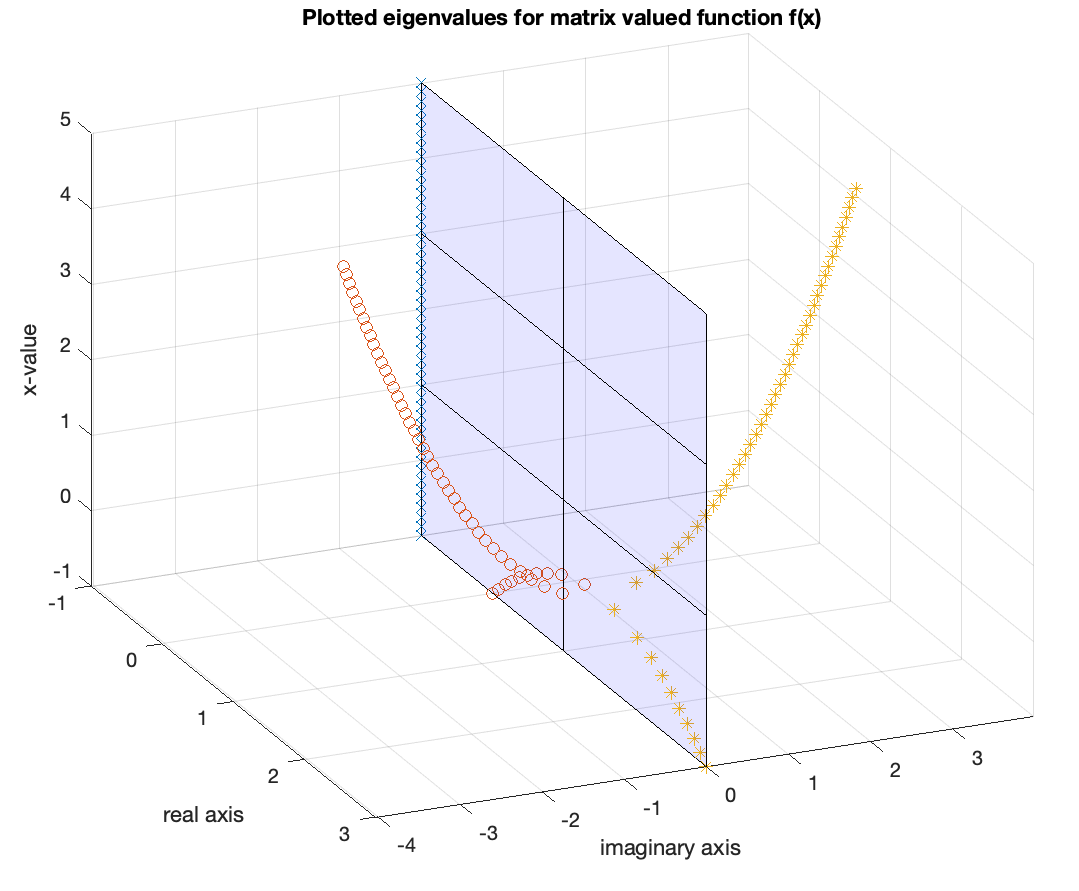
\includegraphics[width=\textwidth]{fig3.png}
        \end{center}
      \end{figure}
\vspace{.15in}

\item[\textbf{(b)}] By doing a by-hand calculation, at what $x$ value in the interval $[-1, 5]$
do non-real eigenvalues first appear? 
\solution 
Forming the characteristic equation like before we get that, 
  \begin{equation*}
   (A - \lambda I) =  \begin{bmatrix}
      2 - \lambda & x & x\\
      -1& -\lambda & 1\\
      -1 & 1 & -\lambda
    \end{bmatrix}
  \end{equation*}
  Solving for $\lambda$ when the determinant is zero we get, 
  \begin{align*}
    \det(A - \lambda I) &= (2 - \lambda)(\lambda^2 - 1) - x(\lambda + 1) + x(-1 - \lambda),\\ 
    &= (2 - \lambda)(\lambda^2 - 1) - 2x(\lambda + 1),\\ 
    &= (2 - \lambda)(\lambda - 1)(\lambda + 1) - 2x(\lambda + 1),\\
    &= (\lambda + 1)((2 - \lambda)(\lambda - 1) - 2x),\\
    &= (\lambda + 1)(-\lambda^2 + 3\lambda - 2(x + 1)).
  \end{align*}
  Applying the quadratic formula we get that in order to have complex eigenvalues the following expression must hold, 
  \begin{align*}
    9 - 4(-1)(-2(x + 1)) &< 0,\\
    9 - 8x - 8 &<0,\\
    x &> \frac{1}{8}. 
  \end{align*}

  \begin{figure}[H]
    \begin{center}
      \caption{The teal plane depicts $x = \frac{1}{8}$.}
      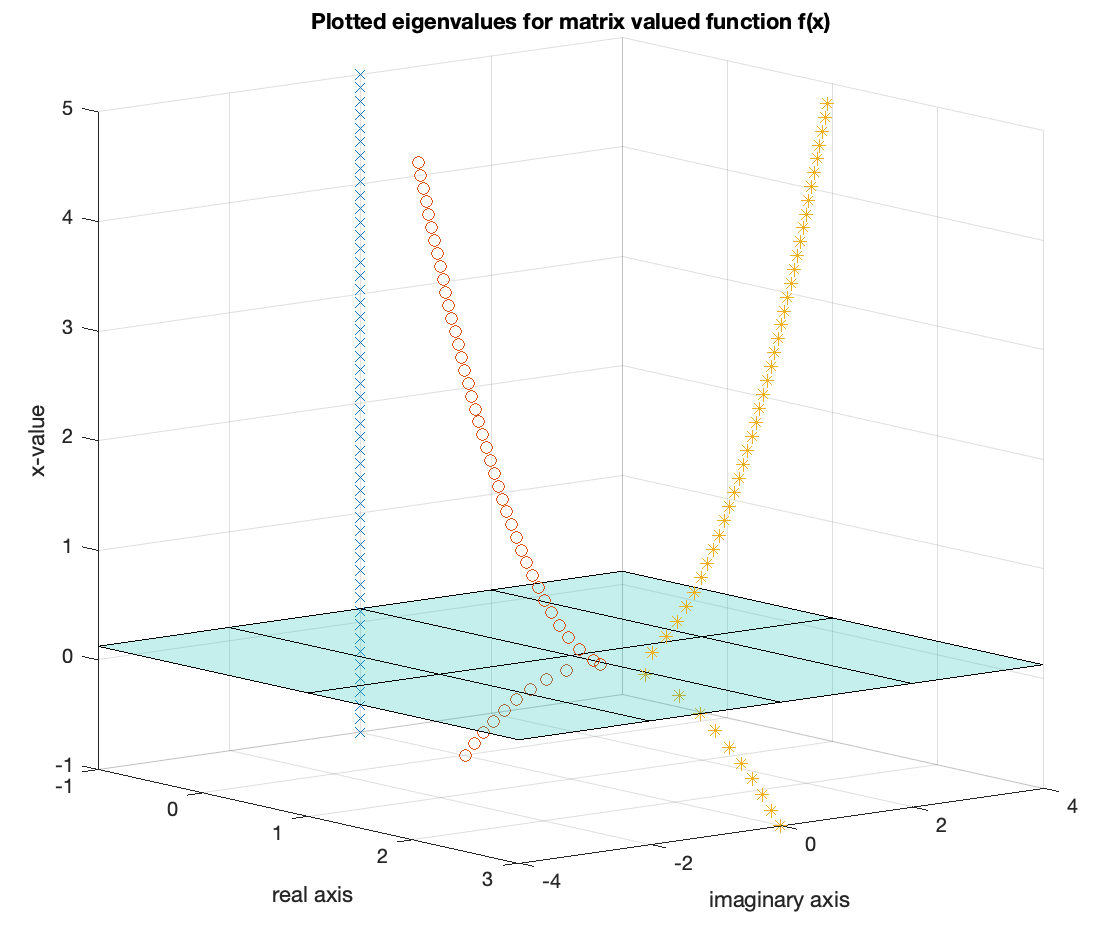
\includegraphics[width=\textwidth]{fig2.png}
    \end{center}
  \end{figure}
\end{enumerate}  
\end{exercise}
\vspace{1in}




\begin{exercise}{Problem P24} Check that the solution $u(t)$ given by Duhamel's principle, equation (5.8)
  in the textbook, satisfies ODE(5.6) and the initial condition $u(t_0) = \eta$.
  \solution Recall that ODE(5.6) is a constant coefficient linear system where $A \in \RR^{S \times S}$ 
 is constant,  
  \begin{equation*}
    u'(t) = Au(t) + g(t).
  \end{equation*} 
  Also recall that the solution given by Duhamel's principle is given by, 
  \begin{equation*}
    u(t) = e^{A(t - t_0)}\eta + \int_{t_0}^{t}e^{A(t - \tau)}g(\tau)d\tau.
  \end{equation*}
  To verify this solution we must first solve for $u'(t)$. Clearly the first part of the sum differentiates to, 
  \begin{equation*}
    u'(t) = Ae^{A(t - t_0)}\eta + \frac{\delta}{\delta t}\left(\int_{t_0}^{t}e^{A(t - \tau)}g(\tau)d\tau\right)
  \end{equation*}
  One can see this by considering the Taylor series definition of the matrix exponential. 
  %% Maybe put it in maybe not.


  Applying a special case of the Leibniz Integral rule, 
  \begin{equation}
    \frac{\delta}{\delta x} \left(\int_a^x f(x, t) dt \right) = f(x, x) + \int_a^x \frac{\delta}{\delta x} f(x, t) dt,
  \end{equation}
  we get the following, 
  \begin{align*}
    \frac{\delta}{\delta t}\left(\int_{t_0}^{t}e^{A(t - \tau)}g(\tau)d\tau\right)&= e^{A(t - t)}g(t) +  \int_{t_0}^{t} \frac{\delta}{\delta t} \left(e^{A(t - \tau)}g(\tau)\right)d\tau\\
    &= (1)g(t) + \int_{t_0}^{t} Ae^{A(t - \tau)}g(\tau) d\tau\\
    &= g(t) + A \int_{t_0}^{t} e^{A(t - \tau)}g(\tau) d\tau
  \end{align*}
  Finally by substitution we get, 
\begin{align*}
  u'(t) &= Ae^{A(t - t_0)}\eta + g(t) + A \int_{t_0}^{t} e^{A(t - \tau)}g(\tau) d\tau,\\
  &= A\left(e^{A(t - t_0)}\eta + \int_{t_0}^{t} e^{A(t - \tau)}g(\tau) d\tau\right) + g(t),\\
  &= Au(t) + g(t).
\end{align*}
\end{exercise}
\vspace{1in}

\begin{exercise}{Problem P25} Consider the ODE system
  \begin{equation*}
    u'_1 = 2u_1,
  \end{equation*}
  \begin{equation*}
    u'_2 = 3u_1 - 2u_2
  \end{equation*}
  with some initial conditions at $t = 0$: $u_1(0) = a$, $u_2(0) = b$.
  
  Solve this system in two ways:
  
  \begin{enumerate}
    \item[\textbf{(a)}] Solve the first equation. Then insert this into the second equation to get a 
    non-homogenous linear ODE for $u_2$. Solve using Duhamel's principle. \\
    \solution Clearly the first equation's solution is $u_1 = ae^{2t}$. Substitution into the second 
    equation gives, 
    \begin{equation*}
      u'_2 = -2u_2 + 3ae^{2t}.
    \end{equation*}
    Applying Duhamel's principle we get, 
    \begin{align*}
      u_2 &= e^{-2t}b + \int_{0}^{t} e^{-2(t - \tau)} (3ae^{2\tau}) d\tau,\\
      &= be^{-2t} + 3a\int_{0}^{t}e^{-2t}e^{2\tau}e^{2\tau} d\tau,\\
      &= be^{-2t} + 3ae^{-2t}\int_{0}^{t}e^{4\tau} d\tau,\\
      &= be^{-2t} + 3ae^{-2t}\left(\frac{1}{4}e^{4t} - \frac{1}{4}\right),\\
      &= be^{-2t} + \frac{3}{4}ae^{2t} - \frac{3}{4}ae^{-2t},
    \end{align*}
    \vspace{.15in}


    \item[\textbf{(b)}] Write the system as $u' = Au$, compute the matrix exponential, and 
    get the solution in the form of equation (D.30) in Appendix D. 
    \solution Written as a system, we get the following, 
    \begin{equation*}
      u' = \begin{bmatrix}
        2 & 0\\
        3 & -2
      \end{bmatrix}
      u,
    \end{equation*}
    \begin{equation*}
      u(0) = \eta = \begin{bmatrix}
        a\\
        b
      \end{bmatrix}.
    \end{equation*}
    Computing the eigendecomposition of $A$ we first note that it's eigenvalues are $\lambda = 2, -2$ since it forms the following
    characteristic equation, $0 = (2 - \lambda)(-2 - \lambda)$. 
    Solving for the associated eigenvectors we get, 
    \begin{align*}
      \begin{bmatrix}
        0 & 0\\
        3 & -4
      \end{bmatrix}
      v_2 = \begin{bmatrix}
        0\\
        0
      \end{bmatrix}\\
      v_2 = \begin{bmatrix}
        1\\
        \frac{3}{4}
      \end{bmatrix}
    \end{align*}
    \begin{align*}
      \begin{bmatrix}
        2 & 0\\
        3 & 0
      \end{bmatrix}
      v_{-2} = \begin{bmatrix}
        0\\
        0
      \end{bmatrix}\\
      v_{-2} = \begin{bmatrix}
        0\\
        1
      \end{bmatrix}
    \end{align*}
    Forming $R$ and $\Lambda$ we get
    \begin{equation*}
      R = \begin{bmatrix}
        1 & 0\\
        \frac{3}{4} & 1
      \end{bmatrix},\qquad
      \Lambda = \begin{bmatrix}
        2 & 0\\
        0 & -2
      \end{bmatrix}
    \end{equation*}
    Solving for $R^{-1}$ we get, 
    \begin{equation*}
      R^{-1} = \begin{bmatrix}
        1 & 0\\
        -\frac{3}{4} & 1
      \end{bmatrix}
    \end{equation*} 
    From (D.30) in Appendix $D$ we can now form the matrix exponential and 
    solve our ODE system,
    \begin{equation*}
      u(t) = e^{At}\eta = (R e^{\Lambda r} R^{-1}) \eta = 
      \begin{bmatrix}
        1 & 0\\
        \frac{3}{4} & 1
      \end{bmatrix}
      \begin{bmatrix}
        e^{2t} & 0\\
        0 & e^{-2r}
      \end{bmatrix}
      \begin{bmatrix}
        1 & 0\\
        -\frac{3}{4} & 1
      \end{bmatrix}
      \begin{bmatrix}
        a\\
        b
      \end{bmatrix}.
    \end{equation*}
    Simplifying we get the same solution as part (a), 
    \begin{align*}
      u(t) &= 
      \begin{bmatrix}
        1 & 0\\
        \frac{3}{4} & 1
      \end{bmatrix}
      \begin{bmatrix}
        e^{2t} & 0\\
        0 & e^{-2r}
      \end{bmatrix}
      \begin{bmatrix}
        a\\
        -\frac{3}{4}a + b
      \end{bmatrix},\\
      &= 
      \begin{bmatrix}
        1 & 0\\
        \frac{3}{4} & 1
      \end{bmatrix}
      \begin{bmatrix}
        ae^{2t}\\
        -\frac{3}{4}ae^{-2t} + be^{-2t}
      \end{bmatrix},\\
      &= 
      \begin{bmatrix}
        1 & 0\\
        \frac{3}{4} & 1
      \end{bmatrix}
      \begin{bmatrix}
        ae^{2t}\\
        -\frac{3}{4}ae^{-2t} + be^{-2t}
      \end{bmatrix},\\
      &=
      \begin{bmatrix}
        ae^{2t}\\
        \frac{3}{4}ae^{2t}-\frac{3}{4}ae^{-2t} + be^{-2t}
      \end{bmatrix}.
    \end{align*}
  \end{enumerate}
\end{exercise}
\vspace{1in}




\begin{exercise}{Problem P26} The ODE IVP
  \begin{equation*}
    v'' = -9v, \qquad v(0) = v_0, \qquad v'(0) = w_0
  \end{equation*}
  has solution, 
  \begin{equation*}
    v(t) = v_0\cos(3t) + \frac{w_0}{3}\sin(3t).
  \end{equation*}
  Verify this. 

  Construct this solution by first rewriting the ODE as a first order system $u' = Av$.
  Then compute the solution $u(t) = e^{At}u(0)$ by using equation (D.30) in Appendix D 
  \solution We begin by first converting this second order ODE IVP into a system of first order ODE
  IVP. Consider the following substitution, and note that $u_1(0) = v_0$ and $u_2(0) = w_0$
  \begin{equation*}
    u_1 = v
  \end{equation*}
  \begin{equation*}
    u_2 = v'
  \end{equation*}
  Differentiating and by substitution we get the following system of differential equations, 
  \begin{equation*}
    u_1' = v' = u_2
  \end{equation*}
  \begin{equation*}
    u_2' = v'' = -9v = -9u_1
  \end{equation*}
  Written out as a system and reordering the rows we get, 
  \begin{equation*}
    \begin{bmatrix}
      u_2'\\
      u_1'
    \end{bmatrix} = \begin{bmatrix}
      0 & 1\\
      -9 & 0
    \end{bmatrix}
    u
  \end{equation*}
  \begin{equation*}
    \eta = \begin{bmatrix}
      v_0\\
      w_0
    \end{bmatrix}.
  \end{equation*}
  Note that we get eigenvalues $\lambda = 3i, -3i$ since the characteristic equation is of the form $(\lambda^2 - (-3)^2)$.
  Consider $\lambda = 3i$ and solving for the corresponding eigenvector we get, 
  \begin{align*}
    \begin{bmatrix}
      -3i & 1\\
      -9 & -3i
    \end{bmatrix}
    v_{3i} &=
    \begin{bmatrix}
      0\\
      0
    \end{bmatrix},\\
    \begin{bmatrix}
      -3i & 1\\
      0 & 0
    \end{bmatrix}
    v_{3i} &=
    \begin{bmatrix}
      0\\
      0
    \end{bmatrix},\\
    v_{3i} &= 
    \begin{bmatrix}
      -\frac{i}{3}\\
      1
    \end{bmatrix}.
  \end{align*} 
Now with $\lambda = -3i$ we get, 
  \begin{align*}
    \begin{bmatrix}
      3i & 1\\
      -9 & 3i
    \end{bmatrix}
    v_{-3i} &=
    \begin{bmatrix}
      0\\
      0
    \end{bmatrix},\\
    \begin{bmatrix}
      3i & 1\\
      0 & 0
    \end{bmatrix}
    v_{-3i} &=
    \begin{bmatrix}
      0\\
      0
    \end{bmatrix},\\
    v_{-3i} &= 
    \begin{bmatrix}
      \frac{i}{3}\\
      1
    \end{bmatrix}.
  \end{align*}
  Note we can now construct the following, 
  \begin{equation*}
    R = \begin{bmatrix}
      -\frac{i}{3} & \frac{i}{3}\\
      1 & 1
    \end{bmatrix},
    \qquad
    \Lambda = 
    \begin{bmatrix}
      3i & 0\\
      0 & -3i
    \end{bmatrix}.
  \end{equation*}
  Solving for $R^{-1}$ we get, 
  \begin{equation*}
    R^{-1} = \frac{1}{-2i/3} \begin{bmatrix}
      1 & -\frac{i}{3}\\
      -1 & -\frac{i}{3}
    \end{bmatrix} = \frac{3i}{2} \begin{bmatrix}
      1 & -\frac{i}{3}\\
      -1 & -\frac{i}{3}
    \end{bmatrix} = 
    \begin{bmatrix}
      \frac{3i}{2} & \frac{1}{2}\\
      -\frac{3i}{2} & \frac{1}{2}
    \end{bmatrix}
  \end{equation*}
  Having diagonalized our matrix we can proceed by forming the solution with equation (D.30) in Appendix D we get, 
  \begin{equation*}
    u = e^{At}\eta = (R e^{\Lambda r} R^{-1}) \eta =  \begin{bmatrix}
      -\frac{i}{3} & \frac{i}{3}\\
      1 & 1
    \end{bmatrix}
    \begin{bmatrix}
      e^{3i} & 0\\
      0 & e^{-3i}
    \end{bmatrix}
    \begin{bmatrix}
      \frac{3i}{2} & \frac{1}{2}\\
      -\frac{3i}{2} & \frac{1}{2}
    \end{bmatrix}
    \begin{bmatrix}
      v_0\\
      w_0
    \end{bmatrix}
  \end{equation*}
  Expanding to check the given solution we get, 
  \begin{align*}
    u &= \begin{bmatrix}
      -\frac{i}{3} & \frac{i}{3}\\
      1 & 1
    \end{bmatrix}
    \begin{bmatrix}
      e^{(3i)t} & 0\\
      0 & e^{(-3i)t}
    \end{bmatrix}
    \begin{bmatrix}
      \frac{(3i)t}{2}v_0 + \frac{1}{2}w_0\\
      -\frac{(3i)t}{2}v_0 + \frac{1}{2}w_0
    \end{bmatrix}\\
    &= \begin{bmatrix}
      -\frac{i}{3} & \frac{i}{3}\\
      1 & 1
    \end{bmatrix}
    \begin{bmatrix}
      e^{(3i)t}(\frac{3i}{2}v_0 + \frac{1}{2}w_0)\\
      e^{(-3i)t}(-\frac{3i}{2}v_0 + \frac{1}{2}w_0)
    \end{bmatrix}\\
    &= \begin{bmatrix}
      -\frac{i}{3} & \frac{i}{3}\\
      1 & 1
    \end{bmatrix}
    \begin{bmatrix}
      e^{(3i)t}(\frac{3i}{2}v_0 + \frac{1}{2}w_0)\\
      e^{(-3i)t}(-\frac{3i}{2}v_0 + \frac{1}{2}w_0)
    \end{bmatrix}
  \end{align*}
  Which gives our solution as, 
  \begin{equation*}
    u_1 = v(t) = \left(-\frac{i}{3}\right)e^{(3i)t}\left(\frac{3i}{2}v_0 + \frac{1}{2}w_0\right) + \left(\frac{i}{3}\right)e^{(-3i)t}\left(-\frac{3i}{2}v_0 + \frac{1}{2}w_0\right)
  \end{equation*}
  Applying Euler's formula and simplifying we get the desired solution, 
  \begin{align*}
    v(t) &= \left(\frac{i}{3}\right)\left(-e^{(3i)t}\left(\frac{3i}{2}v_0 + \frac{1}{2}w_0\right) + e^{(-3i)t}\left(-\frac{3i}{2}v_0 + \frac{1}{2}w_0\right)\right)\\
    &= \left(\frac{i}{3}\right)\left(-(\cos(3t) + i\sin(3t))\left(\frac{3i}{2}v_0 + \frac{1}{2}w_0\right) + (\cos(-3t) + i\sin(-3t))\left(-\frac{3i}{2}v_0 + \frac{1}{2}w_0\right)\right)\\
    &= \left(\frac{i}{3}\right)\left((-\cos(3t) - i\sin(3t))\left(\frac{3i}{2}v_0 + \frac{1}{2}w_0\right) + (\cos(3t) - i\sin(3t))\left(-\frac{3i}{2}v_0 + \frac{1}{2}w_0\right)\right)\\
    &= \left(\frac{i}{3}\right)\left(-2\frac{3i}{2}v_0\cos(3t) - iw_0\sin(3t)\right)\\
    &= v_0\cos(3t) + \frac{w_0}{3}\sin(3t).
  \end{align*}




  
\end{exercise}
















\end{document}











 




